%%%%%%%%%%%%%%%%%%%%%%%%%%%%%%%%%%%%%%%%%%%%%%%%%%%%%%%%%%%%%%%%%
%%% COSYNE-2007 Abstract Template
%%% Version 1.0
%%%%%%%%%%%%%%%%%%%%%%%%%%%%%%%%%%%%%%%%%%%%%%%%%%%%%%%%%%%%%%%%%

\documentclass[12pt,draft]{article}
\usepackage{times}
%\inner 0.5in
\oddsidemargin -0.5in		% margin, in addition to 1" standard
\textwidth 7.5in		% 8.5" - 2*(1+\oddsidemargin)

\topmargin -1in		% in addition to 1.5" standard margin
\textheight 9.75in 		% 11 - ( 1.5 + \topmargin + <bottom-margin> )

\columnsep 0.25in

\parindent 0pt
\parskip 12pt

\flushbottom \sloppy
\pagestyle{empty} % No page numbers

\usepackage{subfigure}
\usepackage{tikz}
\usepackage[sorting=none]{biblatex}
\usepackage{csquotes}
%\usepackage[footnotesize]{caption}


\bibliography{biblio}
%%%%%%%%%%% BEGIN METADATA %%%%%%%%%%%%
\newcommand{\AuthorAG}{Antoine Grimaldi}

\newcommand{\AuthorLP}{Laurent Perrinet}
\newcommand{\AuthorVB}{Victor Boutin}
\newcommand{\AddressLP}{Institut de Neurosciences de la Timone (UMR 7289); Aix Marseille Univ, CNRS; Marseille, France}%
\newcommand{\WebsiteLP}{https://laurentperrinet.github.io}%
\newcommand{\EmailLP}{Laurent.Perrinet@univ-amu.fr}%
\newcommand{\EmailRB}{xxx@xxx}%
\newcommand{\AuthorSI}{Sio-Hoi Ieng}
\newcommand{\AuthorRB}{Ryad Benosman}%
\newcommand{\orcidRB}{0000-0003-0243-944X}%
\newcommand{\AddressRB}{Sorbonne Université, INSERM, CNRS, Institut de la Vision, France;}%
\newcommand{\Abstract}{
A single paragraph of about 200 words maximum. For research articles, abstracts should give a pertinent overview of the work. We strongly encourage authors to use the following style of structured abstracts, but without headings: (1) Background: Place the question addressed in a broad context and highlight the purpose of the study; (2) Methods: Describe briefly the main methods or treatments applied; (3) Results: Summarize the article's main findings; and (4) Conclusion: Indicate the main conclusions or interpretations. The abstract should be an objective representation of the article, it must not contain results which are not presented and substantiated in the main text and should not exaggerate the main conclusions.
}

\begin{document}

%%%----------------------------------------------------------------- 
{\Large\bf  
Image classification using SNN
}

{\bf
\AuthorAG\ , \AuthorVB\ , \AuthorLP\ ,\AuthorSI\ and \AuthorRB}

{ 
Institut de Neurosciences de la Timone, Aix Marseille Univ / CNRS, Marseille, France.
}

%%%----------------------------------------------------------------- 
%%SUMMARY

\parindent 12pt

\textbf{Summary}. 

%%END OF SUMMARY



\begin{figure}[!ht]%[!ht][!b]%
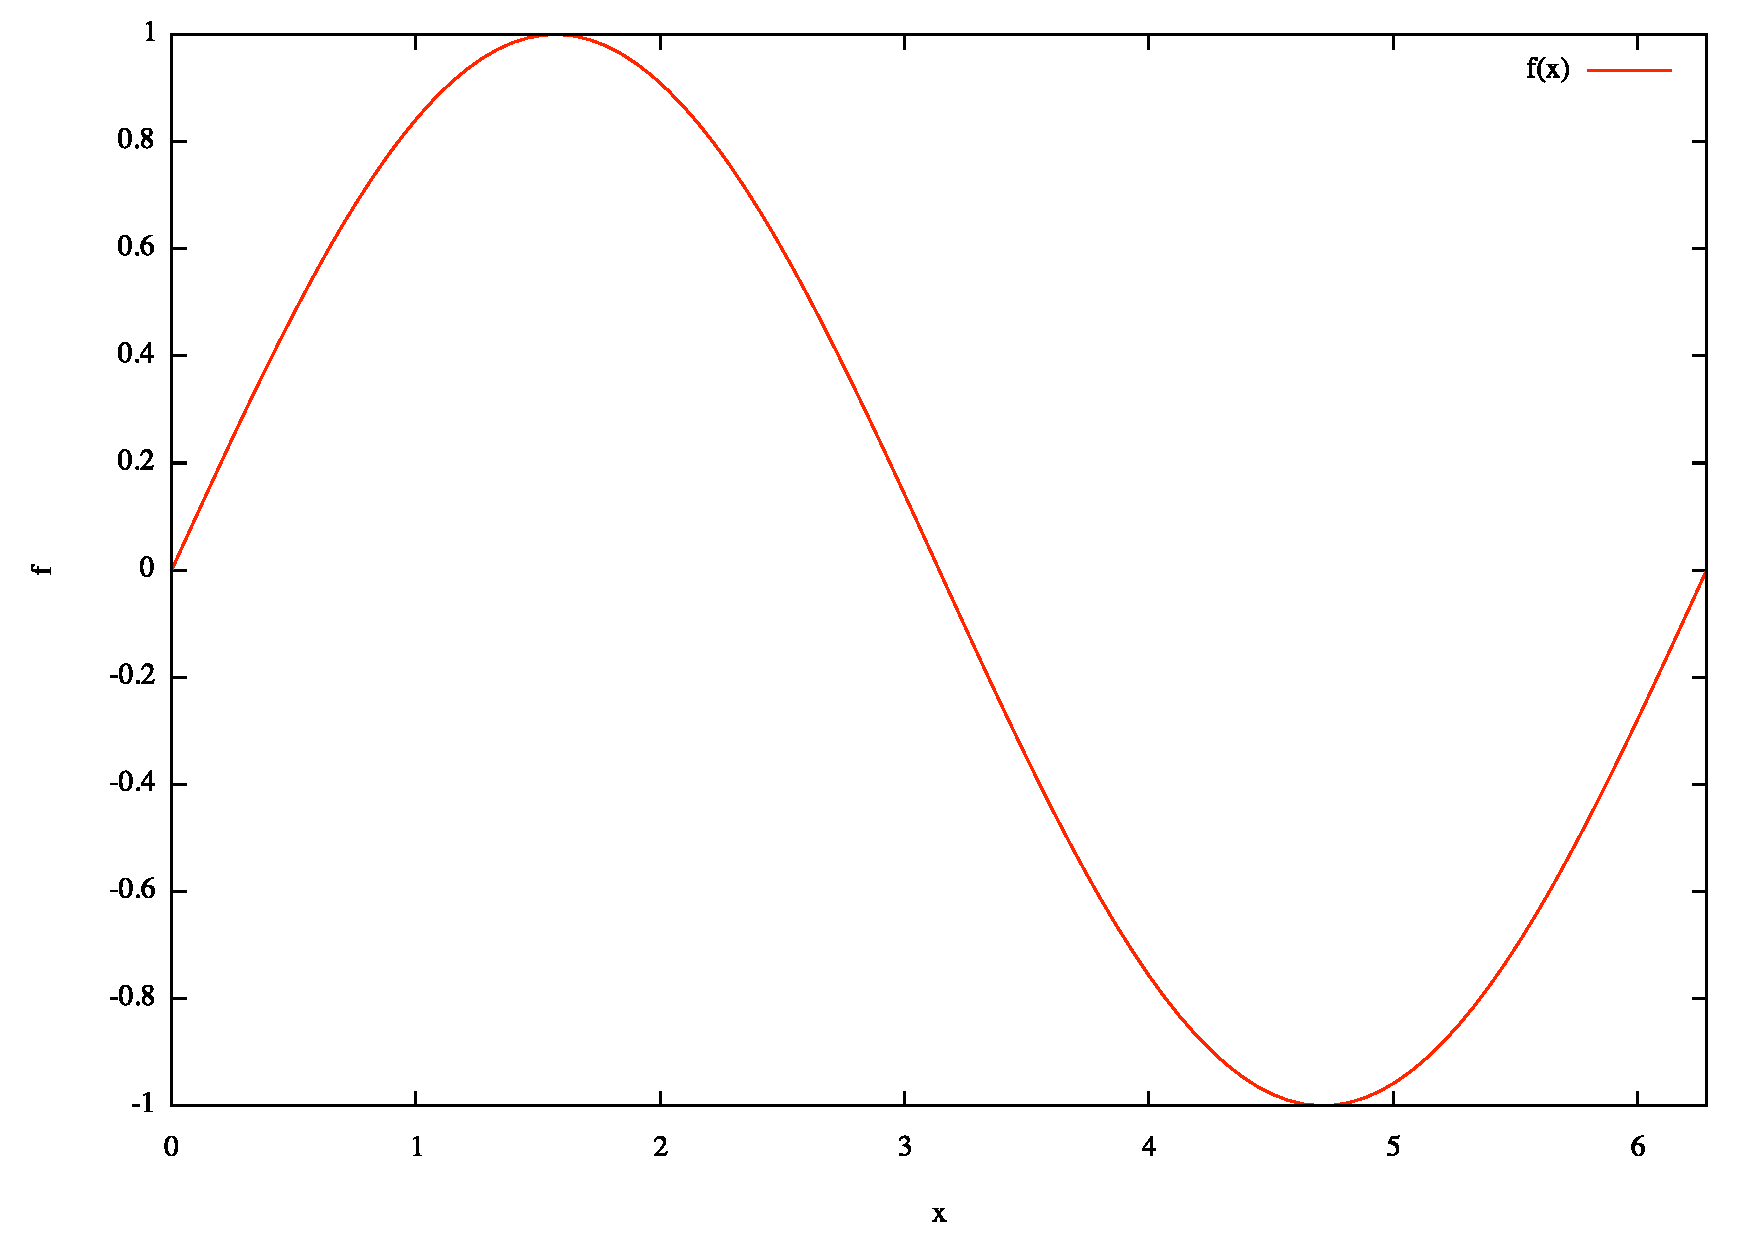
\includegraphics[width=0.99\linewidth]{figure1}
\end{figure}

\caption
{
\textbf{Figure 1}: (a) 
%\label{fig:fig1}
}


\vfil 

%%%----------------------------------------------------------------- 
%{\bf Acknowledgments}\\
%We thank T. Colleague for helpful discussions.  
%This work was supported by NIH grant DC999999.

%%%----------------------------------------------------------------- 
\printbibliography

\end{document}